\chapter{Neural networks (part 2): training in practice}\label{ch-08}

With backpropagation
(\href{07\%20-\%20Note\%20sulla\%20backpropagation}{07 - Notes on
backpropagation}) we know how to compute the gradient for each weight
of the network. This lecture addresses all the practical issues needed
to actually train an MLP: initialisation, multiple minima,
on-line/batch/mini-batch versions, learning rate and momentum, stopping
criteria, overfitting and regularisation, number of units (with Cascade
Correlation), input and output representation. It closes with a summary
of the strengths and weaknesses of neural networks and the first advice
for the project (MONK benchmark).

\begin{figure}[htbp]
\centering
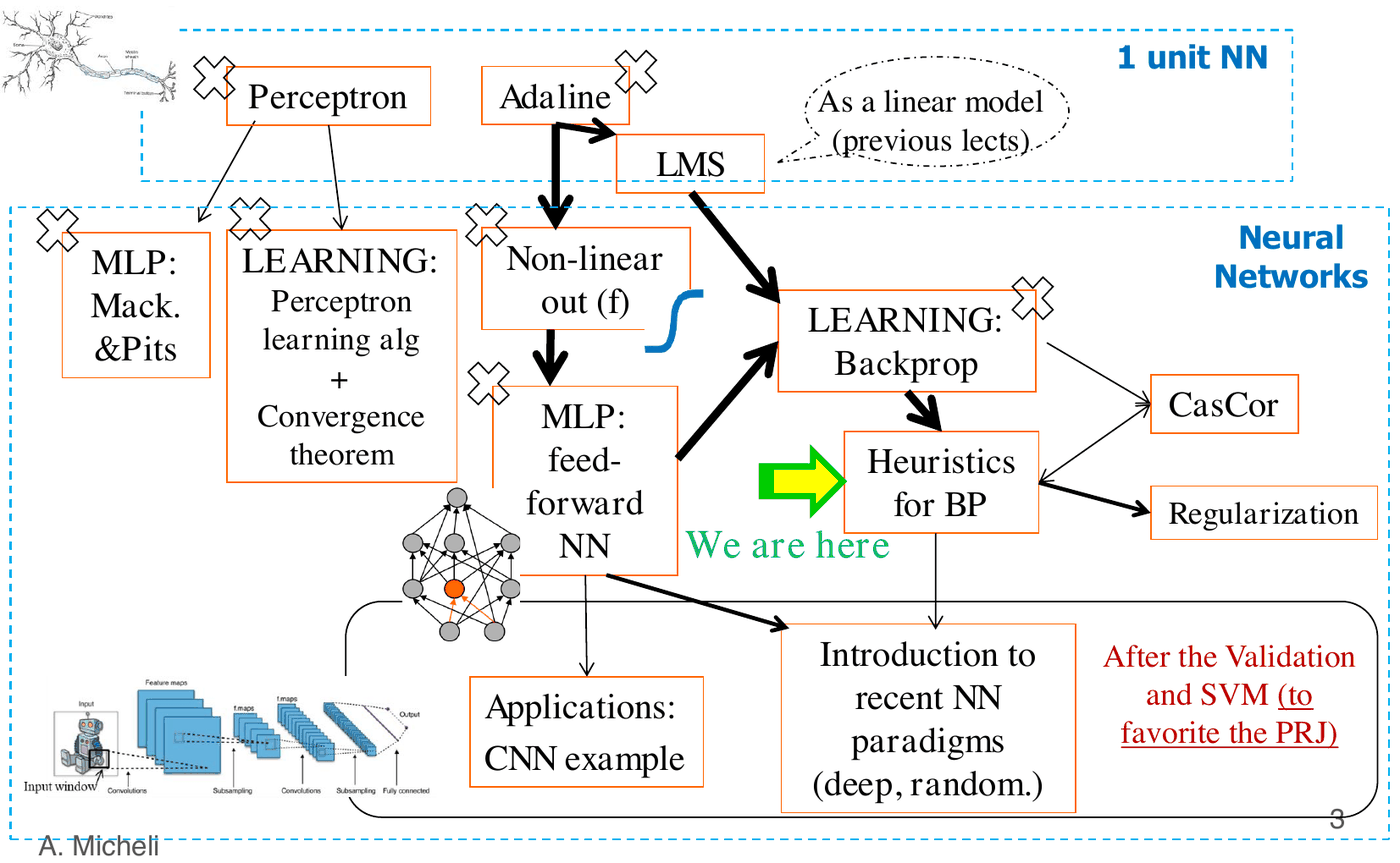
\includegraphics[width=0.91\linewidth,height=0.42\textheight,keepaspectratio]{images/08-nn2_mappa.png}
\caption{Zoom on the ``neural networks'' block of the course.}
\end{figure}

\section{Philosophy}\label{filosofia}

ML has evolved from a collection of heuristic tricks to general
conceptual frameworks: the professor prefers not to introduce too many
heuristic details. Many of the techniques that follow can be explored
experimentally in the project; some have a theoretical foundation
(regularisation) and apply in a more general framework. Those marked
with \textbf{(!)} are very common and \textbf{must be used} in the
project.

\begin{boxwarning}{Beware of ``rules of thumb''}

Avoid the \emph{rules of thumb} found on blogs, unless they are proven
in scientific papers or their advantage has been verified
experimentally.

\end{boxwarning}

\begin{boxtip}{A useful interpretation}

Backpropagation is a \textbf{path in weight space} (on the loss
surface). The path depends on: the data, the model, the
\textbf{starting point} (initial weights), the \textbf{convergence
speed} and the \textbf{end point} (stopping rule). All these choices
constitute a \textbf{control of the search} in the hypothesis space.

\end{boxtip}

The basic algorithm is still gradient descent: small initial weights,
\(\Delta\mathbf{w} = -\partial E/\partial\mathbf{w}\) (computed with
backprop: forward phase up to the outputs, then backward phase for the
deltas), \(\mathbf{w}_{new} = \mathbf{w} + \eta\,\Delta\mathbf{w}\),
repeat. The model is often \textbf{over-parameterised} and the
optimisation is \textbf{non-convex} and potentially unstable: hence the
issues that follow. The \textbf{hyperparameters} are the values that
must be fixed to run the training.

\section{Initial weight values}\label{valori-iniziali-dei-pesi}

\begin{boxtip}{(!) Initialisation}

Initialise the weights with \textbf{random values close to zero}, for
example in the interval \([-0.7;\ +0.7]\) (for standardised data).

\end{boxtip}

To be avoided:

\begin{itemize}
\tightlist
\item
  \textbf{all zeros}: the deltas of the hidden units would all be zero
  (they depend on the weights towards the output) and the network would
  not learn;
\item
  \textbf{high values}: the sigmoids start \textbf{saturated}, with
  almost zero derivatives and very slow learning;
\item
  \textbf{all equal}: the hidden units remain \textbf{symmetric} (they
  receive the same updates and all compute the same thing). Randomness
  serves to \textbf{break the symmetry}.
\end{itemize}

The \textbf{fan-in} (number of inputs of a unit) can be taken into
account, for example with an interval equal to
\(\text{range}\cdot 2/\text{fan-in}\), but not if the fan-in is too
large and not for the output units (otherwise the deltas start close to
zero). Very popular is the \textbf{Glorot and Bengio} initialisation
(2010): biases at 0 and weights from a uniform distribution in
\([-1/a, +1/a]\) with \(a = \sqrt{\text{fan-in}}\) (or, in later
results, \(a\) also dependent on the fan-out).

\begin{boxnote}{(!) For the project}

A very small network (very few units) can depend strongly on the
initialisation.

\end{boxnote}

\section{Multiple minima}\label{minimi-multipli}

The loss is \textbf{not convex}: there are many local minima, and the
result depends on the initial weights. Therefore:

\begin{boxtip}{(!) Multiple initialisations}

Try several random initial configurations (for example 5--10 or more
\emph{trials}). To evaluate the model, report the \textbf{mean} of the
results (mean of the errors) and the \textbf{variance}. If a single
answer is wanted, one can choose the solution with the lowest
validation error (or the median), or exploit the different end points
with a \textbf{committee} answer (average of the outputs or vote).
Later we will see why \emph{ensembles} are advantageous in general.

\end{boxtip}

Stopping in a local minimum with too high an error is not a big
problem: one sees the final error and can start again. Often a
\textbf{``good'' local minimum is enough}.

\subsection{Do we really need the global
minimum?}\label{serve-davvero-il-minimo-globale}

Two fundamental remarks:

\begin{enumerate}
\def\labelenumi{\arabic{enumi}.}
\tightlist
\item
  In ML \textbf{we look for neither the local nor the global minimum of
  \(R_{emp}\)}, but for the minimum of \(R\), which we cannot compute.
  Often we stop at a point that does not even have zero gradient.
\item
  The network is a \textbf{variable-dimension hypothesis space}: during
  training the VC-dim grows, the training error goes down towards zero
  (or the global minimum) while the network becomes too complex. One
  must stop \textbf{before} this condition of \emph{overtraining} (and
  hence overfitting), regardless of the local/global minima issue.
\end{enumerate}

\section{On-line, batch and mini-batch}\label{on-line-batch-e-mini-batch}

Let us recall (see linear models):

\begin{itemize}
\tightlist
\item
  \textbf{Batch}: the gradients of all patterns of an \textbf{epoch}
  (a complete cycle of presentation of the training set) are summed
  and then the weights are updated.
\item
  \textbf{On-line/stochastic}: \(\mathbf{w}\) is updated after each
  pattern \(p\) with \(\Delta_p\mathbf{w}\), without waiting for the
  sum. It makes progress at every example and can be faster, but it
  requires a smaller \(\eta\).
\end{itemize}

In formulas, for the weight \(w_{tu}\): \[
\text{batch: } -\frac{\partial E}{\partial w_{tu}} = -\sum_{p=1}^{l}\frac{\partial E_p}{\partial w_{tu}} = \sum_{p=1}^{l}\delta_{p,t}\,o_{p,u}, \qquad \text{on-line: } -\frac{\partial E_p}{\partial w_{tu}} = \delta_{p,t}\,o_{p,u}.
\]

\begin{boxabstract}{Batch and on-line compared}

\textbf{Batch} --- 1) fix \(\mathbf{w}_{init}\) and \(\eta\); 2)
compute \(\Delta\mathbf{w}\) on the whole training set (the sum over
\(p\) is inside this step); 3)
\(\mathbf{w}_{new} = \mathbf{w} + \eta\,\Delta\mathbf{w}\); 4) repeat
until convergence.

\textbf{On-line} --- 1) fix \(\mathbf{w}_{init}\) and \(\eta\); for
each pattern \(p\): 2) compute \(\Delta_p\mathbf{w}\); 3)
\(\mathbf{w}_{new} = \mathbf{w} + \eta\,\Delta_p\mathbf{w}\); 4) repeat
(epoch after epoch) until convergence.

\end{boxabstract}

Batch gives a \textbf{more accurate} estimate of the gradient. In
on-line learning the gradient of a single pattern is a \textbf{noisy}
approximation of the overall gradient, hence the name \emph{stochastic
gradient descent}: the descent proceeds in a zig-zag, which \textbf{can
help escape local minima}.

\begin{boxtip}{(!) Shuffling}

In the on-line version the patterns must be presented in a
\textbf{different order} at each epoch (usually by \textbf{shuffling
them randomly}), to avoid a systematic drift in the descent.

\end{boxtip}

\begin{figure}[htbp]
\centering
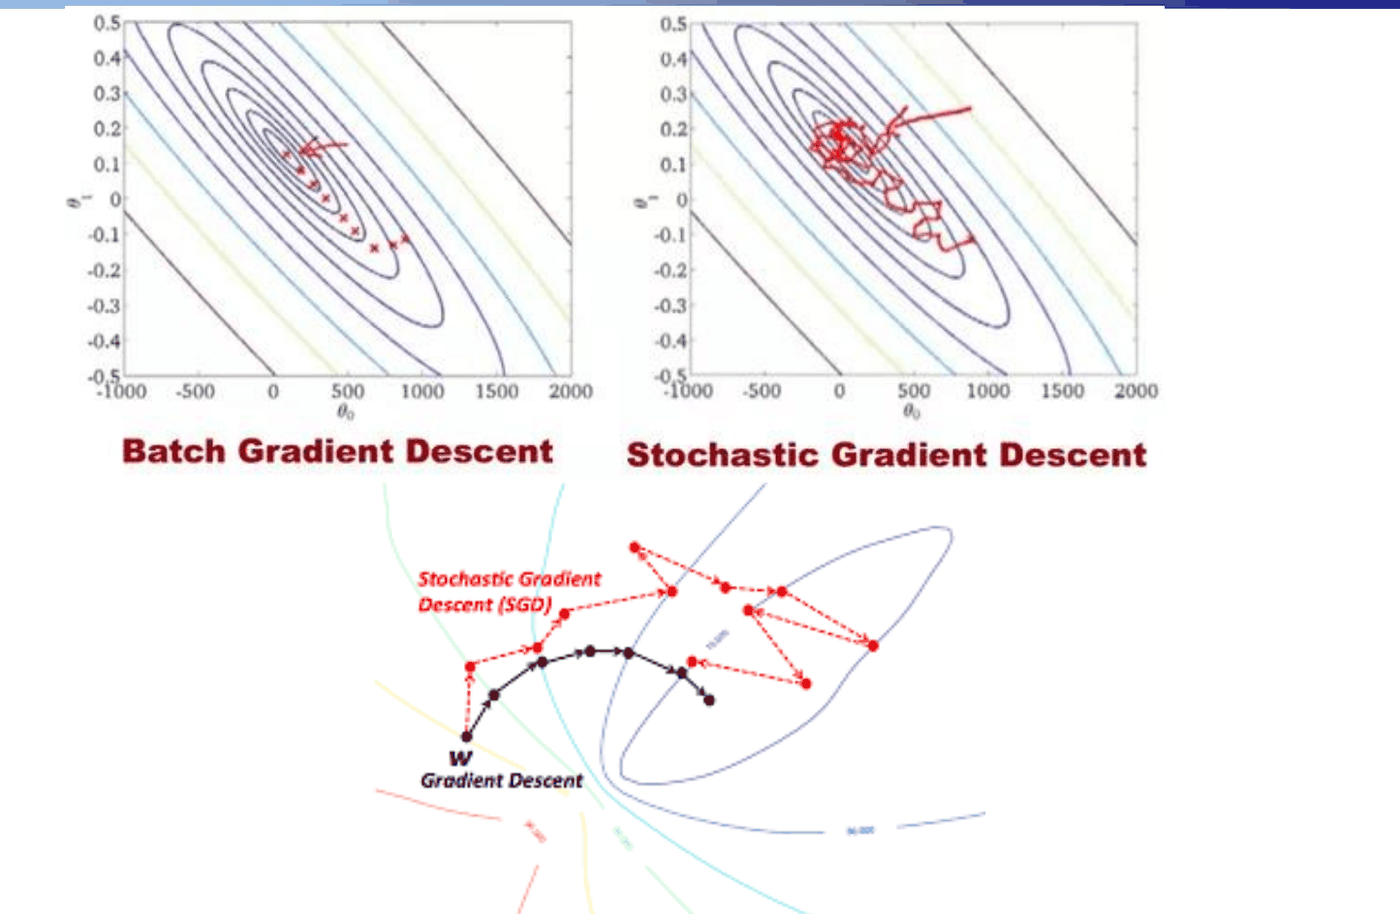
\includegraphics[width=0.71\linewidth,height=0.42\textheight,keepaspectratio]{images/08-nn2_sgd-vs-batch.png}
\caption{Batch and stochastic gradient descent.}
\end{figure}

\subsection{Mini-batch}\label{mini-batch}

In \textbf{mini-batch} each epoch is divided into parts: the gradients
of \(mb\) patterns (\(1 < mb < l\)) are summed before updating the
weights, and this is repeated until all data of the epoch have been
used. The update thus takes place at each mini-batch instead of at each
pattern or each epoch.

\begin{figure}[htbp]
\centering
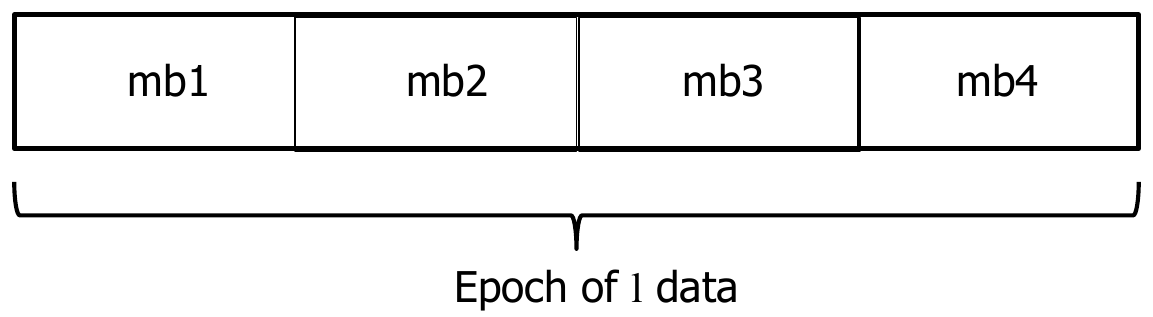
\includegraphics[width=0.60\linewidth,height=0.42\textheight,keepaspectratio]{images/08-nn2_minibatch.png}
\caption{An epoch split into mini-batches.}
\end{figure}

{\def\LTcaptype{none} % do not increment counter
\begin{longtable}[]{@{}
  >{\raggedright\arraybackslash}p{(\linewidth - 4\tabcolsep) * \real{0.3333}}
  >{\raggedright\arraybackslash}p{(\linewidth - 4\tabcolsep) * \real{0.3333}}
  >{\raggedright\arraybackslash}p{(\linewidth - 4\tabcolsep) * \real{0.3333}}@{}}
\toprule\noalign{}
\begin{minipage}[b]{\linewidth}\raggedright
On-line
\end{minipage} & \begin{minipage}[b]{\linewidth}\raggedright
Mini-batch (SGD)
\end{minipage} & \begin{minipage}[b]{\linewidth}\raggedright
Batch
\end{minipage} \\
\midrule\noalign{}
\endhead
\bottomrule\noalign{}
\endlastfoot
does not exploit parallelism across examples & trade-off; fits the GPU
memory & more accurate gradient estimate \\
can be unstable & & slower (waits for all data) \\
noise can have a \textbf{regularising effect} & & \\
\end{longtable}
}

\textbf{Mini-batch SGD} uses random sampling (shuffling) for an
unbiased estimate of the gradient. With huge training sets or streaming
data one can even do without epochs. Since the cost of an update
depends on \(mb\) and not on \(l\), mini-batch SGD is a key factor for
scaling learning to datasets of millions of examples.

\section{\texorpdfstring{The learning rate
\(\eta\)}{The learning rate \textbackslash eta}}\label{il-learning-rate-eta}

\begin{itemize}
\tightlist
\item
  \textbf{Batch}: more accurate gradient → a higher \(\eta\) can be
  used.
\item
  \textbf{On-line}: faster but more unstable → smaller \(\eta\).
\item
  In general: \textbf{high} \(\eta\) is fast but can be unstable;
  \textbf{low} \(\eta\) is stable but can be too slow. Typically it is
  searched in \([0.01;\ 0.5]\) with LMS.
\end{itemize}

\begin{boxtip}{(!) Always look at the learning curve}

The plot of the error during training makes it possible to check the
behaviour in the early design phases. Here the \textbf{quality} of the
curve and the \textbf{speed} of convergence are evaluated (the absolute
value of the error also depends on the capacity of the model and on
the other hyperparameters).

\end{boxtip}

\begin{figure}[htbp]
\centering
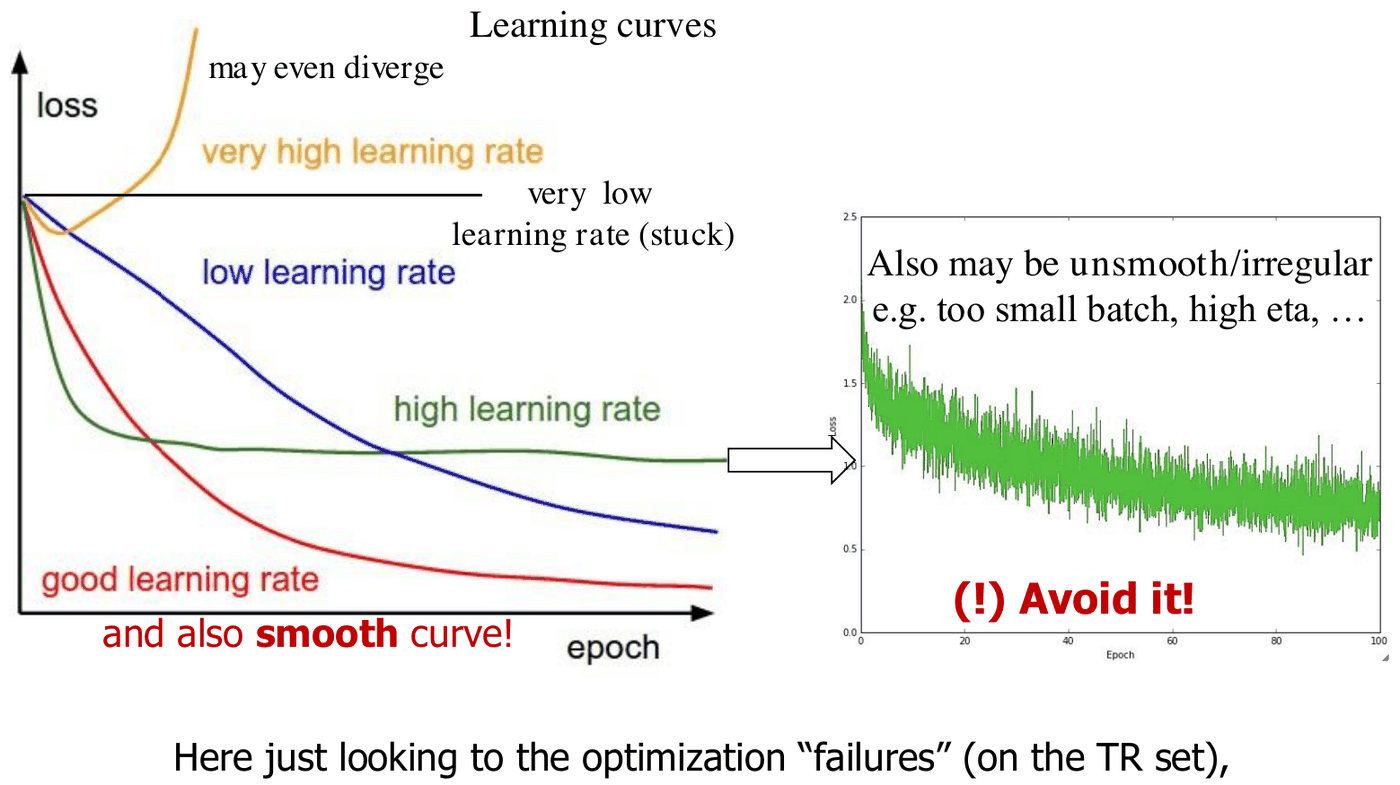
\includegraphics[width=0.91\linewidth,height=0.42\textheight,keepaspectratio]{images/08-nn2_eta.png}
\caption{Effect of the learning rate on the learning curves (training
error).}
\end{figure}

An irregular curve may be due to batches that are too small or to
\(\eta\) too high: it must be avoided. We look for a curve that
decreases quickly \textbf{and smoothly}. (Here we only look at the
``failures'' of the optimisation on the training set, not at the
generalisation error.)

\subsection{\texorpdfstring{LMS: dividing by
\(l\)}{LMS: dividing by l}}\label{lms-dividere-per-l}

\begin{boxtip}{(!) Use the mean of the gradients}

It is convenient to use the \textbf{mean} of the gradients over the
epoch (sum divided by \(l\)): it makes the approach uniform with
respect to the number of data (it is \emph{least mean squares}). It is
equivalent to using \(\eta/l\) with \(0 < \eta < 1\).

Beware: when comparing on-line and batch with LMS, on-line requires a
\textbf{much smaller} \(\eta\) (by the same factor \(1/l\)) to be
comparable. For mini-batch (if dividing by \(mb\)) \(\eta\) must be
re-tuned, or one always divides by \(l\).

\end{boxtip}

\subsection{Improving the descent}\label{migliorare-la-discesa}

\subsubsection{Momentum (!)}\label{momentum}

\[
\Delta\mathbf{w}_{new} = -\eta\,\frac{\partial E(\mathbf{w})}{\partial\mathbf{w}} + \alpha\,\Delta\mathbf{w}_{old}, \qquad \mathbf{w}_{new} = \mathbf{w} + \Delta\mathbf{w}_{new},
\] with \(0 < \alpha < 1\) (for example \(0.5\)--\(0.9\)). Here
\(\eta\) is included in \(\Delta\mathbf{w}\), and after each step
\(\Delta\mathbf{w}_{old} = \Delta\mathbf{w}_{new}\) is saved.

It is the \textbf{``heavy ball'' method}: at each step a fraction of
the previous displacement is added, as if the weights had inertia.

\begin{itemize}
\tightlist
\item
  \textbf{Faster on plateaus}: if the gradient has the same sign in
  consecutive iterations, momentum increases the step.
\item
  \textbf{Dampens oscillations}: in directions in which the gradient
  changes sign the contributions cancel out.
\item
  \textbf{Inertia effect}: allows higher \(\eta\) to be used.
\end{itemize}

\begin{figure}[htbp]
\centering
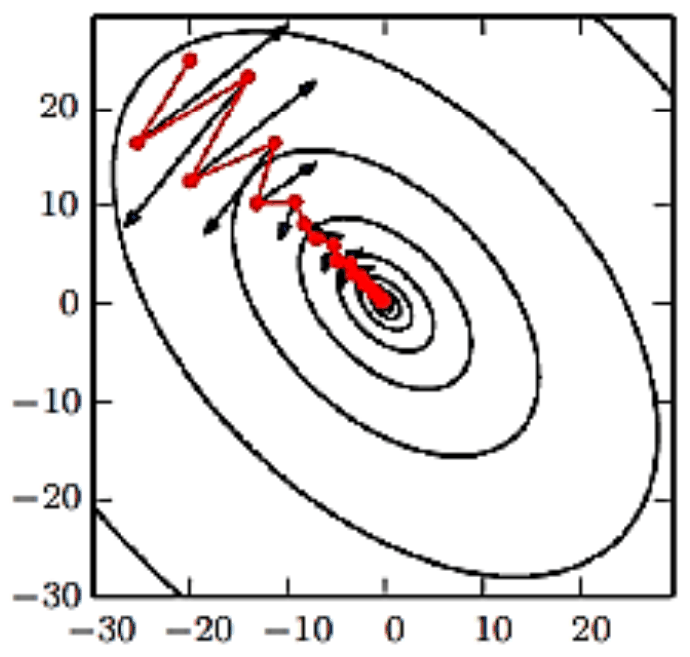
\includegraphics[width=0.46\linewidth,height=0.42\textheight,keepaspectratio]{images/08-nn2_momentum.png}
\caption{Effect of momentum in a ``canyon'' of the error surface
(ill-conditioned Hessian): the red path goes along the valley instead
of bouncing between the walls.}
\end{figure}

Momentum was born for batch. In on-line learning
\(\Delta\mathbf{w}_{old}\) is that of the \textbf{previous pattern},
and momentum becomes a \textbf{moving average of past gradients} that
smooths the stochastic gradients within the epoch (similarly for
mini-batch). The meaning is therefore different from batch, where
gradients computed on the same examples in different epochs are
combined.

\textbf{Nesterov momentum}: momentum is applied first
(\(\mathbf{w} + \alpha\Delta\mathbf{w}_{old}\)), the gradient is
evaluated at this intermediate point, and then the
\(\Delta\mathbf{w}\) (momentum plus new gradient) is applied to the
original weights. It improves the convergence speed in batch (not in
the stochastic case).

\subsubsection{Variable learning rate}\label{learning-rate-variabile}

With mini-batch the gradient \textbf{does not tend to zero} near the
minimum (because of sampling noise), so a fixed \(\eta\) should be
avoided. For example it is decreased linearly until iteration
\(\tau\): \[
\eta_s = \left(1 - \frac{s}{\tau}\right)\eta_0 + \frac{s}{\tau}\,\eta_\tau, \qquad s \le \tau,
\] and then a constant, small \(\eta = \eta_\tau\) is used (for example
\(\eta_\tau \approx 1\%\) of \(\eta_0\), \(\tau\) a few hundred
steps). \(\eta_0\) is chosen with the instability/stall trade-off
(preliminary trials or grid search).

\subsubsection{Adaptive learning rates}\label{learning-rate-adattivi}

Algorithms that automatically adapt the learning rate during training,
even separately \textbf{for each parameter}: \textbf{AdaGrad},
\textbf{RMSProp}, \textbf{Adam} (very popular and often robust with the
default values, but with caution). They are combined with momentum. In
networks with many layers, \(\eta\) can also depend on the layer or on
the fan-in.

\subsection{Beyond basic SGD}\label{oltre-lo-sgd-di-base}

SGD is efficient (linear in the number of parameters) but depends on
the number of data and epochs. There are many heuristics:
\textbf{Quickprop} (jumps to the minimum of a parabola that locally
approximates the loss), \textbf{R-prop} (uses only the \textbf{sign} of
the gradient, not its value, useful when the gradient vanishes in deep
layers).

\textbf{Second-order methods} use the Hessian (second derivatives) to
obtain information about the curvature and descend better (Newton's
method), but the Hessian is extremely expensive. There are approximate
versions: Gauss-Newton, Levenberg-Marquardt, \emph{Hessian-free} methods
such as \textbf{conjugate gradient}, quasi-Newton methods such as
\textbf{BFGS}.

\begin{boxnote}{Saddle points}

A saddle point has (almost) zero gradient but is not a minimum. In
high-dimensional spaces saddle points grow exponentially with respect
to local minima. Newton's method looks for (and ``jumps towards'')
zero-gradient points, so it is more sensitive to saddle points: this
may explain why second-order methods have not replaced gradient descent
for neural networks, while gradient descent empirically manages to
escape saddle points. In practice we find low loss values fairly
quickly, which are mainly useful for generalisation.

\end{boxnote}

\begin{boxtip}{In practice}

For optimisation, the basic approaches (those marked with (!)), if
applied correctly, are usually enough. Experience with well-known
techniques matters more than sophisticated methods one does not know
how to handle. The optimisation technique is relevant only if there are
obstacles to training: \textbf{validation matters more than
optimisation on the training set}, because optimising on the training
data is not our goal. The starting point (also for teaching purposes)
is \textbf{SGD with momentum} (and regularisation).

\end{boxtip}

\section{Stopping criteria}\label{criteri-di-arresto}

\begin{itemize}
\tightlist
\item
  The basic criterion is the error used (mean error \(< \epsilon\)): it
  is the best if the tolerance of the data is known (expert
  knowledge), but often this is not the case. Variants: maximum
  tolerance instead of mean; for classification, the number of errors.
\item
  ``Internal'' criteria: weights that no longer change, almost zero
  gradient (Euclidean norm \(< \epsilon\)), error that no longer
  decreases significantly within an epoch (e.g.\ less than 0.1\%).
  Beware: they can be \textbf{premature} (for example with \(\eta\) too
  small), so \(k\) epochs are observed (\textbf{patience}).
\item
  \textbf{(!)} Stop anyway after an excessive number of epochs, to
  escape overly slow convergence, but \textbf{do not} stop at an
  arbitrary number of epochs fixed a priori.
\item
  And do not necessarily stop with a very low training error\ldots{}
\end{itemize}

\section{Overfitting and
regularisation}\label{overfitting-e-regolarizzazione}

\subsection{Stop at the minimum?}\label{fermarsi-al-minimo}

Typically we do \textbf{not} want the global minimiser of
\(R_{emp}(\mathbf{w})\), because it is probably an overfitting
solution: this is a fundamental difference with respect to optimisation
methods (CM). Our main goal is \textbf{complexity control} to obtain
the best generalisation, through regularisation (explicit with a
penalty term, or implicit with early stopping), plus model selection
(cross-validation) to find the trade-off.

\subsection{How overfitting arises in a
network}\label{come-nasce-loverfitting-in-una-rete}

\begin{itemize}
\tightlist
\item
  We start with \textbf{small random weights} (symmetry breaking).
\item
  The input→output mapping is almost \textbf{linear} (the sigmoids
  work in the linear zone): the effective number of free parameters
  (and the VC-dim) is almost that of a perceptron.
\item
  As optimisation proceeds, the hidden units tend to \textbf{saturate},
  increasing the effective number of parameters and the
  non-linearities: the VC-dim grows.
\end{itemize}

It is again the \textbf{variable-dimension hypothesis space}.

\begin{figure}[htbp]
\centering
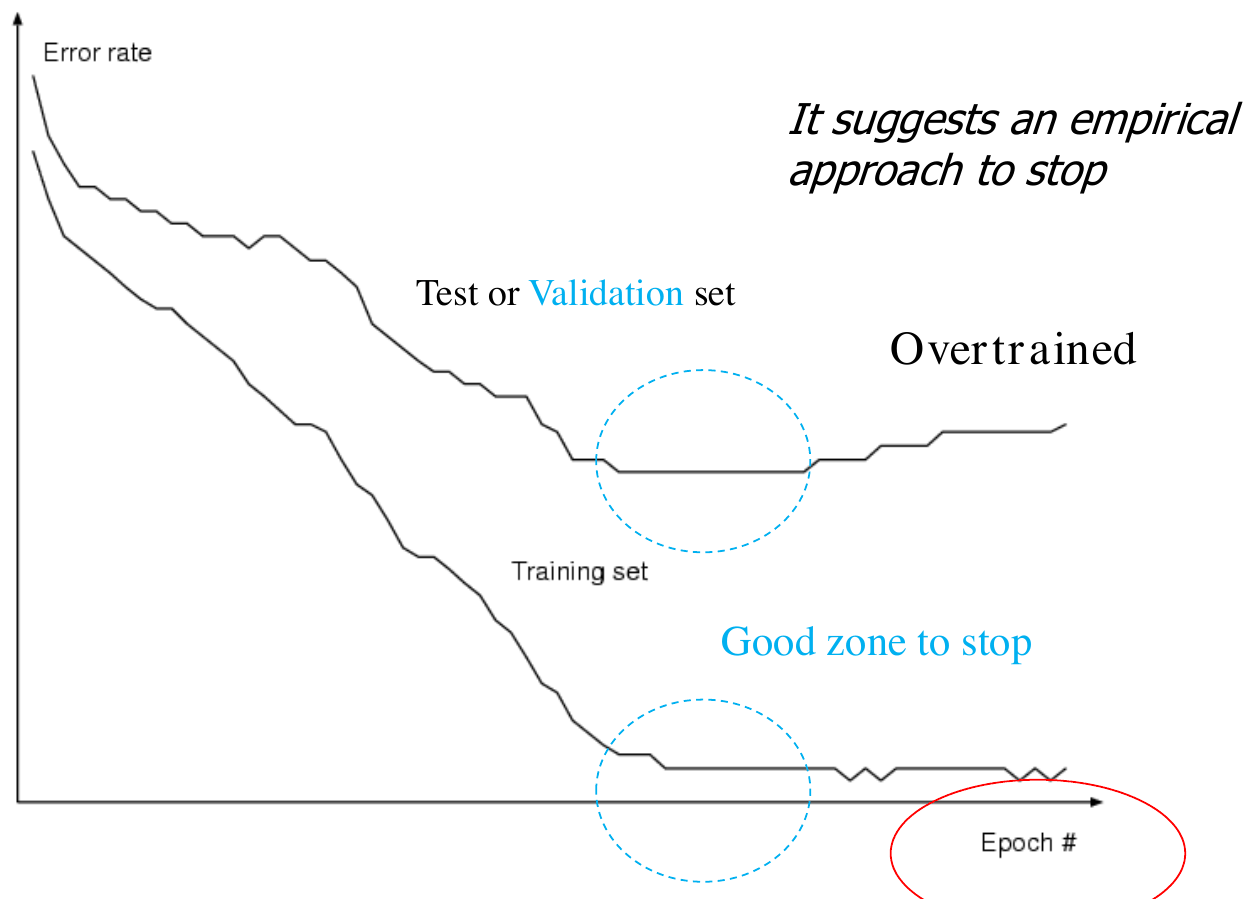
\includegraphics[width=0.63\linewidth,height=0.42\textheight,keepaspectratio]{images/08-nn2_early-stopping.png}
\caption{Typical behaviour of backpropagation: it suggests an empirical
criterion for stopping.}
\end{figure}

The curve must be read together with the VC-bound plot (theoretical
foundation). How to intervene:

\begin{enumerate}
\def\labelenumi{\arabic{enumi}.}
\tightlist
\item
  \textbf{Early stopping}: use a \textbf{validation set} to decide
  when to stop, i.e.\ when the validation error starts to rise. It is
  vague: several epochs must be observed before deciding
  (\emph{patience}) and possibly one must go back
  (\emph{backtracking}). Since the effective number of parameters grows
  during training, \textbf{stopping earlier is equivalent to limiting
  the effective complexity}.
\item
  \textbf{Regularisation} of the loss: our main tool.
\item
  \textbf{Pruning} methods (later).
\end{enumerate}

\subsection{Regularisation (!)}\label{regolarizzazione}

During training the weights grow: we can optimise the loss taking their
value into account. The principled approach (Tikhonov again) adds a
penalty term: \[
\text{Loss}(\mathbf{w}) = \sum_p\big(d_p - o(\mathbf{x}_p)\big)^2 + \lambda\,\|\mathbf{w}\|^2, \qquad \|\mathbf{w}\|^2 = \sum_i w_i^2 \text{ over all the weights of the network.}
\] The effect is \textbf{weight decay}: about \(2\lambda w\) is added
to the gradient of each weight, \[
\mathbf{w}_{new} = \mathbf{w} + \eta\,\Delta\mathbf{w} - 2\lambda\mathbf{w}
\] (the 2 can be omitted). \(\lambda\) is usually very small
(e.g.\ \(0.01\)) and is chosen in \textbf{model selection}
(cross-validation). Applied to a linear model it is ridge regression;
there are more sophisticated penalties (for example for \emph{weight
elimination}).

\begin{boxnote}{Error and Loss}

With a penalty term it is worth distinguishing: \textbf{Loss} is the
objective function used for training (MSE + penalty);
\textbf{Error/Risk} is the data term (MSE), which measures the error of
the model. \textbf{(!)} It is the error that must be reported in tables
and plots, because it is the useful measure for those who use the
model.

\end{boxnote}

\begin{figure}[htbp]
\centering
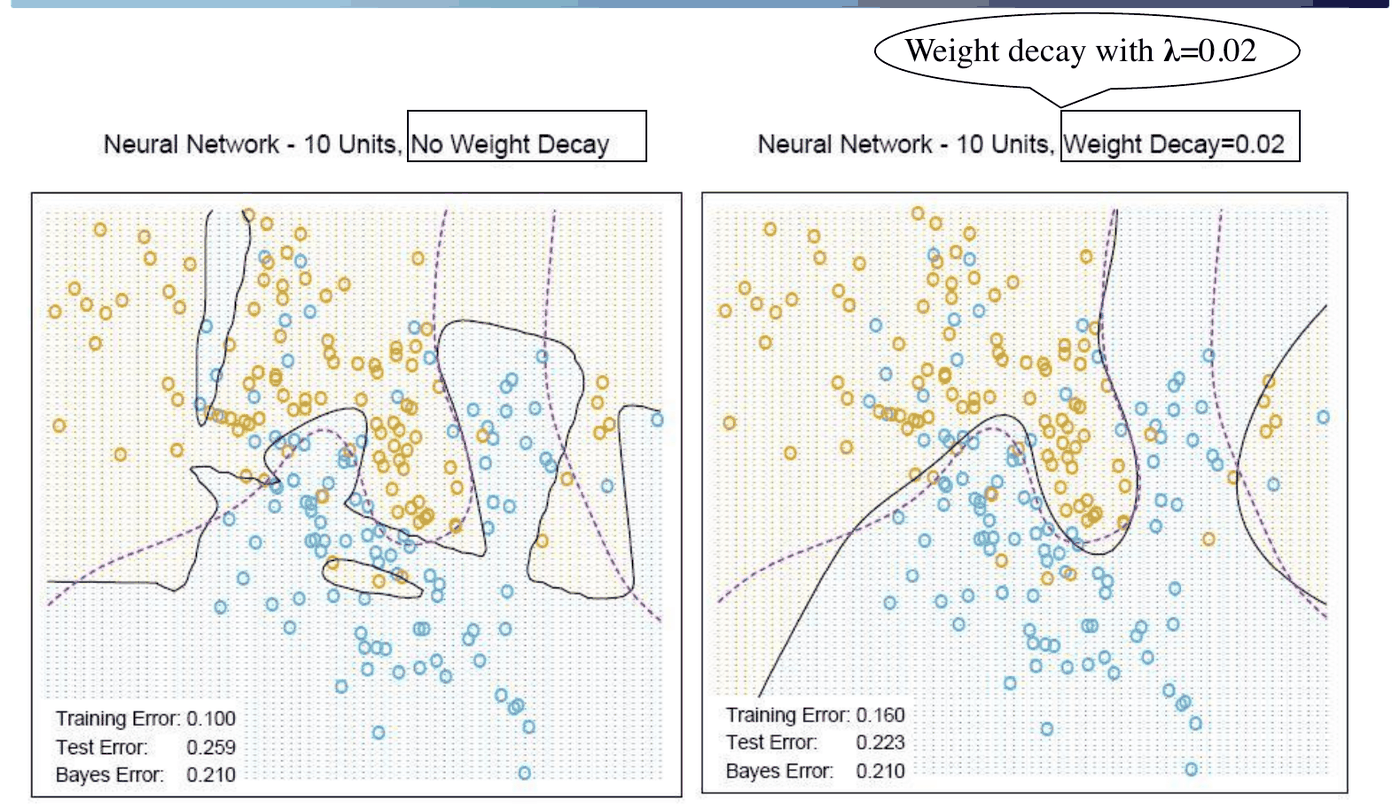
\includegraphics[width=0.91\linewidth,height=0.42\textheight,keepaspectratio]{images/08-nn2_weight-decay.png}
\caption{Effect of weight decay on a 10-unit network
(Hastie-Tibshirani-Friedman): the boundary becomes more regular and the
test error gets closer to the Bayes error (0.210).}
\end{figure}

\begin{figure}[htbp]
\centering
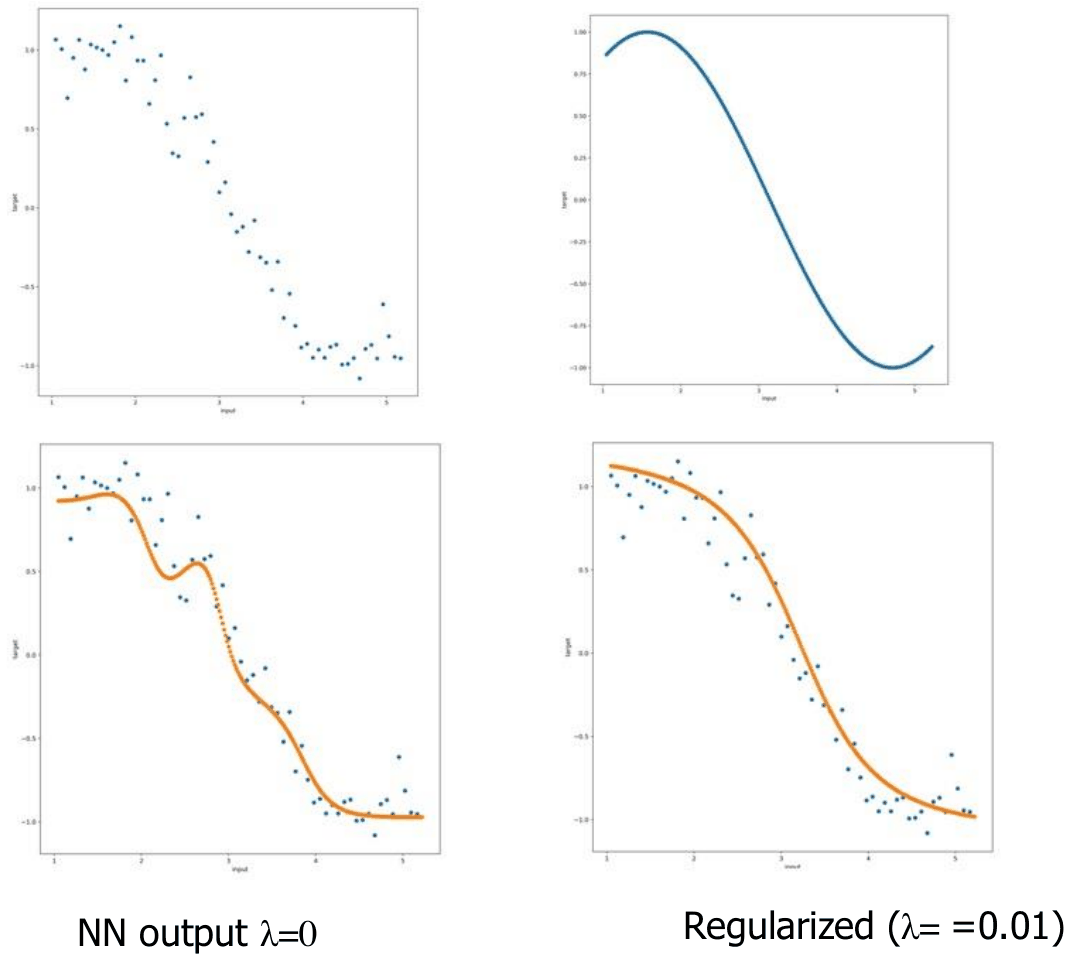
\includegraphics[width=0.63\linewidth,height=0.42\textheight,keepaspectratio]{images/08-nn2_regressione-reg.png}
\caption{Univariate regression: network without regularisation
(\(\lambda = 0\)) and regularised (\(\lambda = 0.01\)).}
\end{figure}

\begin{figure}[htbp]
\centering
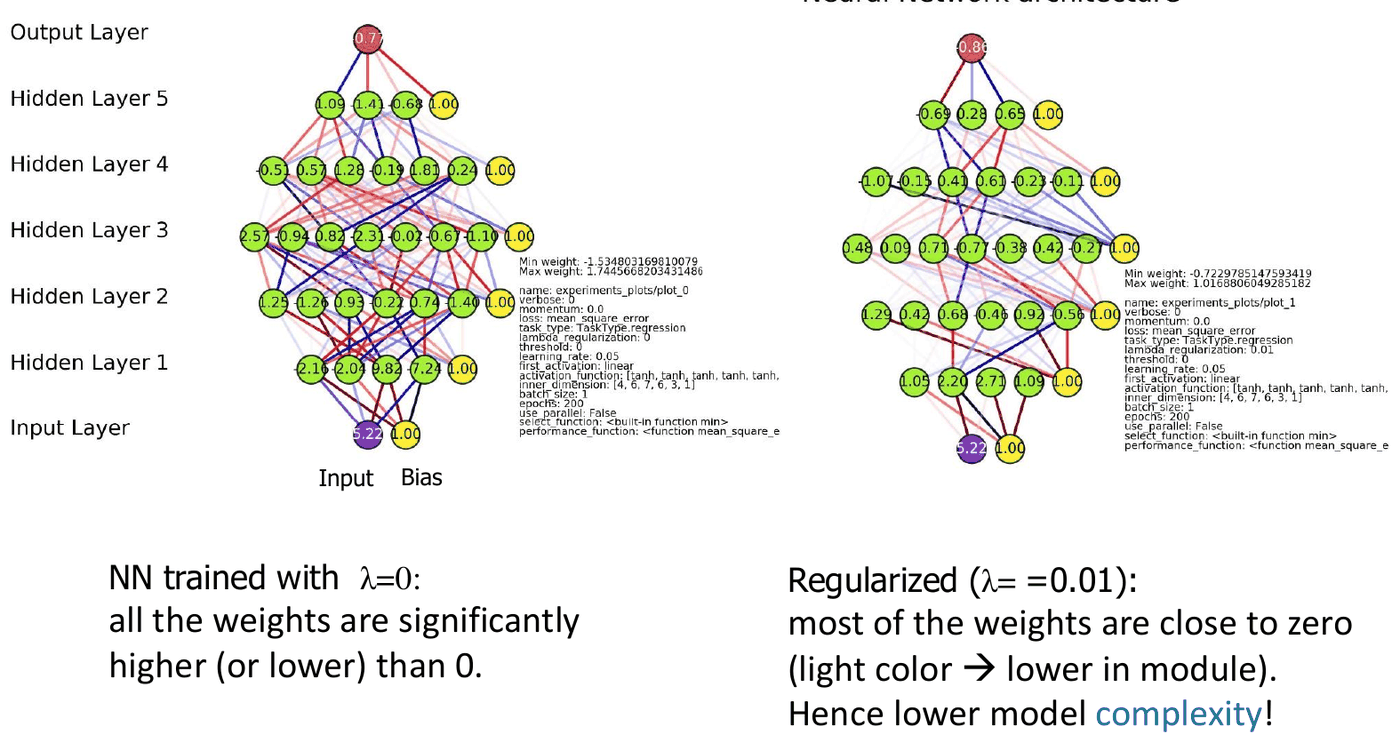
\includegraphics[width=0.91\linewidth,height=0.42\textheight,keepaspectratio]{images/08-nn2_pesi-reg.png}
\caption{The weights of the network without regularisation (left) and
with regularisation (right): with \(\lambda = 0.01\) most weights are
close to zero, so the complexity of the model is lower.}
\end{figure}

\subsubsection{Common
misconceptions}\label{fraintendimenti-frequenti}

\begin{boxwarning}{Regularisation is not for stabilising convergence}

Regularisation is \textbf{not} a technique to make the learning curve
more stable: it serves to \textbf{control the complexity} of the model
(measured by the VC-dim, related to the number and value of the
weights). If the curve is unstable, the problem lies elsewhere
(learning rate, batch\ldots).

\end{boxwarning}

\begin{boxquestion}{Early stopping or regularisation?}

Early stopping is an \textbf{empirical} approach that requires a
validation set to decide when to stop, sacrificing part of the data.
Regularisation in the loss is a \textbf{principled} approach: it allows
the validation curve to follow the training curve (as long as there is
no underfitting due to a too high \(\lambda\)), and in that case early
stopping is not (strictly) needed and one can stop at convergence. Both
can also be used: early stopping does not intervene if the validation
error does not rise.

\end{boxquestion}

\subsubsection{Details}\label{dettagli}

\begin{itemize}
\tightlist
\item
  Often the \textbf{bias \(w_0\) is excluded} from the regulariser
  (including it would make the results dependent on
  translations/scalings of the target), or it has its own coefficient.
\item
  It is typically applied in the batch version. In on-line/mini-batch
  the penalty is applied at every step, hence many times per epoch: for
  a fair comparison with batch one would use \(\lambda\cdot mb/l\). (If
  \(\lambda\) is chosen with model selection, this happens
  automatically.)
\item
  Another technique is \textbf{dropout} (later).
\end{itemize}

\subsection{Putting everything together: momentum and weight
decay}\label{mettere-tutto-insieme-momentum-e-weight-decay}

With the regularised loss, the rule with momentum becomes (separating
the two terms of the loss and using \(\eta\) only for the error term,
as already done for linear models): \[
\Delta w_{tu} = -\eta\,\frac{\partial\,\text{Loss}}{\partial w_{tu}} + \alpha\,\Delta w_{tu}^{old} \;\doteq\; \eta\,\delta_t\,o_u - \lambda\,w_{tu} + \alpha\,\Delta w_{tu}^{old}, \qquad w_{tu}^{new} = w_{tu} + \Delta w_{tu}.
\] In this way \(\eta\) does not multiply \(\lambda\): changing one
does not change the other.

Should momentum also include the \(\lambda\) part? Often yes (Matlab,
Caffe\ldots). But to make \textbf{all three hyperparameters} \(\eta\),
\(\alpha\), \(\lambda\) \textbf{independent} one can write: \[
\Delta w_{tu} = \eta\,\delta_t\,o_u + \alpha\,\Delta w_{tu}^{old}, \qquad w_{tu}^{new} = w_{tu} + \Delta w_{tu} - \lambda\,w_{tu},
\] separating weight decay from the momentum memory. Only the gradient
of \(E\) (where the sum over patterns is) is divided by \(l\).

\section{Number of hidden units}\label{numero-di-unituxe0-nascoste}

The number of units is related to \textbf{complexity control}, to the
input dimension and to the size of the training set. In general it is
a \textbf{model selection} problem: the number of units, together with
\(\lambda\), is chosen with cross-validation.

\begin{itemize}
\tightlist
\item
  Too few units → underfitting; too many → overfitting (it can
  happen).
\item
  The number of units can be higher if adequate regularisation is
  used.
\end{itemize}

Alternatives to manual search:

\begin{itemize}
\tightlist
\item
  \textbf{constructive approaches}: the algorithm decides the number of
  units starting from a small network and adding more;
\item
  \textbf{pruning methods}: one starts from large networks and
  progressively removes weights or units.
\end{itemize}

\subsection{Cascade Correlation}\label{cascade-correlation}

Among constructive approaches (Tower, Tiling, Upstart for
classification) the best known is \textbf{Cascade Correlation} (CC) by
Fahlman and Lebiere (1990), for regression and classification. It
learns \textbf{both the weights and the topology} (number of units):
the hypothesis space has a flexible dimension, decided by the
algorithm, and at each step only one unit is trained.

\begin{boxabstract}{Cascade Correlation algorithm}

\begin{enumerate}
\def\labelenumi{\arabic{enumi}.}
\tightlist
\item
  Start from a network \(N_0\) \textbf{without hidden units} and train
  it. If it does not solve the problem, move to \(N_1\).
\item
  In \(N_1\) a hidden unit is added whose weights are trained to
  \textbf{maximise the correlation} between its output and the
  \textbf{residual error} of network \(N_0\).
\item
  After training, the input weights of the new unit are
  \textbf{frozen}; the remaining weights (output layer) are retrained.
\item
  If the network does not solve the problem, more units are added,
  each connected to \textbf{all the inputs and all the previous hidden
  units} (hence ``cascade'').
\item
  Continue until the residual error satisfies the stopping criterion.
\end{enumerate}

\end{boxabstract}

\begin{figure}[htbp]
\centering
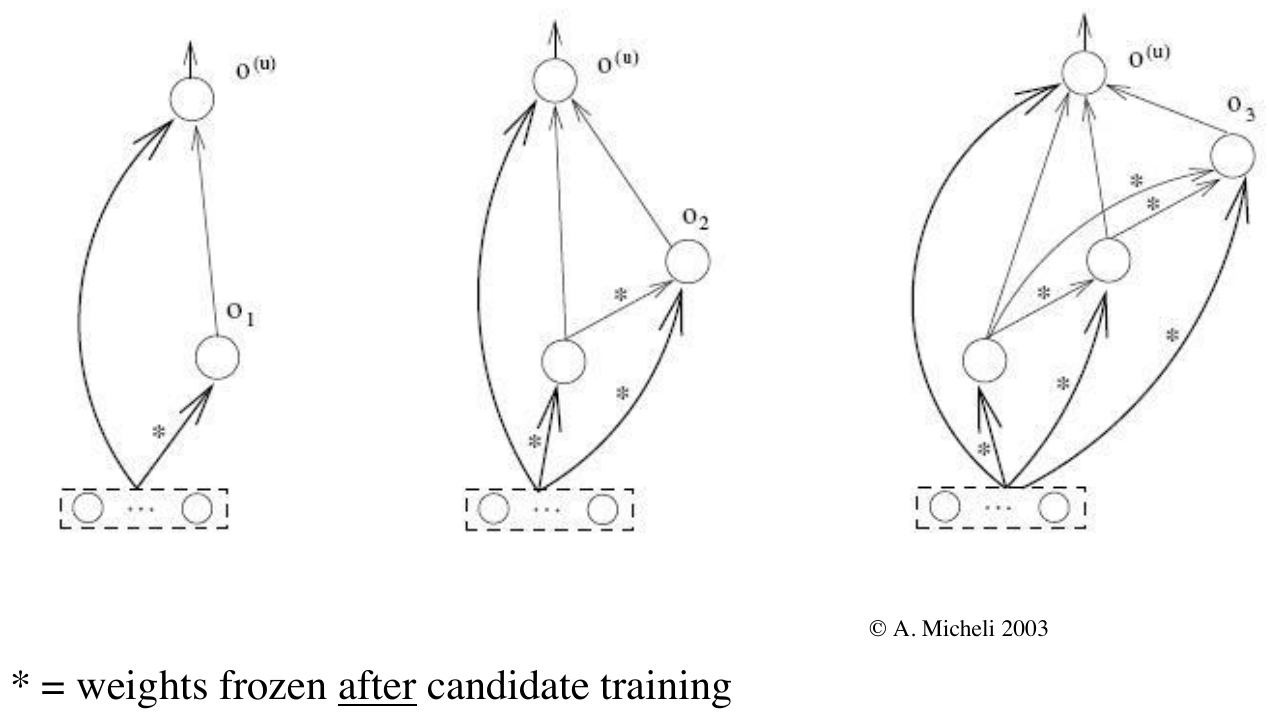
\includegraphics[width=0.74\linewidth,height=0.42\textheight,keepaspectratio]{images/08-nn2_cascade.png}
\caption{Construction of a Cascade Correlation network with up to 3
hidden units.}
\end{figure}

The algorithm alternates minimisation of the total error (LMS, for
example backprop on the output layer) and \textbf{maximisation of the
covariance} \(S\) between the output \(o_p\) of the candidate and the
residual error \(E_{p,k} = o_{p,k} - d_{p,k}\): \[
S = \sum_k\left|\sum_p\big(o_p - \bar{o}\big)\big(E_{p,k} - \bar{E}_k\big)\right|.
\] The gradient (with \(d|f|/dx = \operatorname{sign}(f)\,df/dx\) and
neglecting the dependence of the means on \(o_p\)) is \[
\frac{\partial S}{\partial w_j} = \sum_k \operatorname{sgn}(S_k)\sum_p\big(E_{p,k} - \bar{E}_k\big)\,f'(net_{p,h})\,I_{p,j},
\] where \(h\) is the candidate and \(I_{p,j}\) its input \(j\).
Gradient \textbf{ascent} is performed (\(S\) is maximised).

Notes on CC:

\begin{itemize}
\tightlist
\item
  the role of the hidden units is to \textbf{reduce the residual
  error}: each unit solves a sub-problem and becomes a
  \textbf{permanent feature detector};
\item
  \textbf{candidate pool}: the surface of \(S\) has many maxima, so a
  group of candidates is trained and the best one is chosen, avoiding
  local maxima;
\item
  it is a \textbf{greedy} algorithm: it converges easily and can find a
  minimal number of units, but it can overfit (regularisation is
  needed);
\item
  the loss does not necessarily have to be ``max \(S\)'' (for
  regression LMS can be used).
\end{itemize}

\section{Input and output}\label{input-e-output}

\textbf{Input}: pre-processing has a big effect.

\begin{itemize}
\tightlist
\item
  \textbf{Standardisation} (often useful): for each feature mean 0 and
  standard deviation 1, \((v - \text{mean})/\text{std.\ dev.}\).
\item
  \textbf{Rescaling} to \([0,1]\): \((v - \min)/(\max - \min)\).
\item
  Categorical inputs: \textbf{1-of-K} encoding (\(A \to 100\),
  \(B \to 010\), \(C \to 001\)).
\item
  Missing data: beware, \textbf{0 does not mean ``no input''} if 0 is
  within the range of values.
\end{itemize}

\textbf{Output}:

\begin{itemize}
\tightlist
\item
  \textbf{(!) Regression}: \textbf{linear} output units (one or more).
\item
  \textbf{Classification}: one unit (binary) or 1-of-K with several
  outputs. With the sigmoid, the threshold for assigning the class is
  chosen (with a possible rejection zone); with 1-of-K the highest
  output wins. Often \textbf{tanh} (symmetric) learns faster. As target
  one can use \(0.9\) instead of 1 (and \(-0.9\) or \(0.1\) instead of
  \(-1\) or \(0\)) to avoid asymptotic convergence towards saturation.
  Obviously the range of the targets must lie within the range of the
  outputs.
\item
  \textbf{Softmax} for multi-class 0/1 targets: the outputs sum to 1
  and can be interpreted as probabilities
  \(p(\text{class} = k \mid \mathbf{x})\): \[
  o_k(\mathbf{x}) = \frac{e^{net_k}}{\sum_{j=1}^{K} e^{net_j}}.
  \]
\item
  \textbf{Cross-entropy} can be used as an alternative loss (maximum
  likelihood estimation); for one unit: \[
  -\sum_{i \in TR}\big\{d_i\log(out(\mathbf{x}_i)) + (1 - d_i)\log(1 - out(\mathbf{x}_i))\big\}.
  \]
\end{itemize}

\begin{boxquestion}{Exercise for the project}

Reflect on the role of the different hyperparameters and relate them to
the theory: for example relate the loss with penalty to the VC-bound,
to understand how the number of units, \(\lambda\) and the others
control underfitting and overfitting. Which are the most relevant for
the project (and for winning the competition)?

\end{boxquestion}

\section{Strengths and weaknesses of neural
networks}\label{pregi-e-difetti-delle-reti-neurali}

\begin{boxabstract}{Strengths}

\begin{itemize}
\tightlist
\item
  Flexible method: it extends linear methods to the estimation of
  arbitrary functions and builds an \textbf{explicit hypothesis}
  (unlike K-NN).
\item
  Expressive power given by number of units, architecture and
  training.
\item
  Rich, continuous hypothesis space, differentiable loss → training
  with gradient descent.
\item
  Universal approximators; they handle noise and incomplete data with
  graceful degradation; continuous and discrete data, regression and
  classification.
\item
  A broad \textbf{paradigm} (also unsupervised learning, associative
  memories, stochastic approaches).
\item
  Neural plausibility; \textbf{distributed representation} of
  knowledge (compact in weight matrices); \textbf{fault tolerance};
  adaptation to non-stationary environments with on-line learning
  (\emph{continual learning}, with the stability-plasticity dilemma).
\end{itemize}

\end{boxabstract}

\begin{boxwarning}{Critical points}

\begin{itemize}
\tightlist
\item
  \textbf{Black box problem}: it is difficult to interpret the acquired
  knowledge and extract it for human experts. It is related to the
  current topic of \textbf{explainable AI} (XAI). Approaches:
  projection/clustering of internal representations, sensitivity
  analysis, \textbf{Layer-wise Relevance Propagation} (LRP, 2015, also
  for deep networks, which produces heat maps on the parts of the input
  relevant to the decision), extraction of symbolic rules.
\item
  \textbf{Architecture design}: constructive/pruning methods or
  different approaches (SVM) are needed.
\item
  \textbf{Dependence on the training process}: the many variants and
  hyperparameters affect the final solution.
\item
  Not ideal with \textbf{missing data} (removal, imputation\ldots{} are
  used).
\end{itemize}

\end{boxwarning}

Neural networks are appropriate when: the input is high-dimensional
(discrete or real), the task is classification or regression, the data
may be noisy, training time is not critical, the form of the target
function is unknown, readability of the result is not critical, and the
output computation must be fast.

\begin{boxnote}{Historical notes}

McCulloch and Pitts (1943), Hebb (1949), Minsky (1954, 1969), von
Neumann (1956), Rosenblatt (1958), Widrow and Hoff (1960), Kohonen
(1972, 1982), Grossberg (ART, 1980), Hopfield (1982), Rumelhart,
Hinton, Williams, Werbos, Parker, LeCun (1975--1985, backprop), Poggio
and Girosi (RBF theory, 1990), Vapnik (SVM, 1990s), deep learning
(Hinton, Bengio, LeCun, since 2007). \textbf{Hopfield and Hinton}
received the \textbf{2024 Nobel Prize in Physics}; Hinton, Bengio and
LeCun the 2018 Turing Award.

\end{boxnote}

\section{Towards the project: the MONK
benchmark}\label{verso-il-progetto-il-benchmark-monk}

We are not yet ready for the project (\textbf{validation} and the
dedicated lecture are still missing), but one can start implementing
the network (backprop and update rules) or exploring the simulators.

Verifying the correctness of an implementation is difficult: a network
often ``works'' (even if badly) despite small errors. The first test is
the \textbf{MONK} dataset (UCI), whose results must be reported in the
report:

\begin{itemize}
\tightlist
\item
  3 binary classification tasks, small and artificial, ``not
  difficult'': a small network with few units reaches very high
  accuracies (up to 100\%) in little time;
\item
  there is a report with previous results of MLPs and other models;
\item
  \textbf{input}: 6 variables with 2, 3 or 4 symbolic values each →
  \textbf{1-of-k} encoding → \textbf{17 input units};
\item
  the test set includes the training set (bad practice, but irrelevant
  here).
\end{itemize}

\begin{boxtip}{Tips for the first trials on MONK}

\begin{itemize}
\tightlist
\item
  One output unit for classification (targets and outputs consistent,
  \(0/1\) or \(-1/+1\)); \textbf{tanh} at the output is suggested.
\item
  \textbf{One-hot encoding of the inputs}: a very frequent mistake if
  forgotten!
\item
  Batch with gradient divided by the number of patterns: it converges
  in a few hundred epochs.
\item
  Few hidden units (2--5), as in the manual: the test works if
  state-of-the-art results are reached with few units.
\item
  MONK is sensitive to initialisation (few units): try small initial
  intervals (or fan-in based).
\item
  With on-line approaches use \textbf{shuffling} (the patterns are
  ordered by class).
\end{itemize}

\end{boxtip}

Good results on MONK \textbf{do not guarantee} the correctness of the
simulator; bad results \textbf{surely} indicate that code or settings
must be revised. In the plots what matters is the \textbf{shape} of the
curves (smooth, converging), not the values.

\begin{figure}[htbp]
\centering
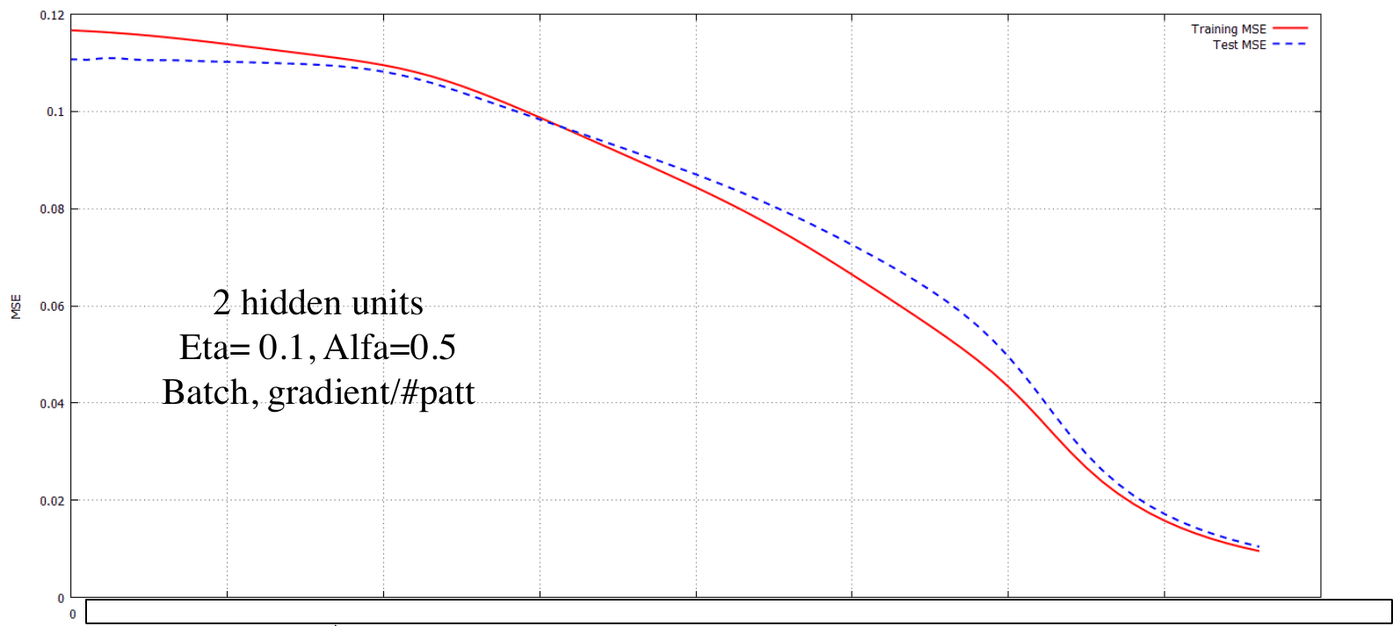
\includegraphics[width=0.80\linewidth,height=0.42\textheight,keepaspectratio]{images/08-nn2_monk2-mse.png}
\caption{MONK2: training (red) and test (dashed blue) MSE with 2 hidden
units, \(\eta = 0.1\), \(\alpha = 0.5\).}
\end{figure}

\begin{figure}[htbp]
\centering
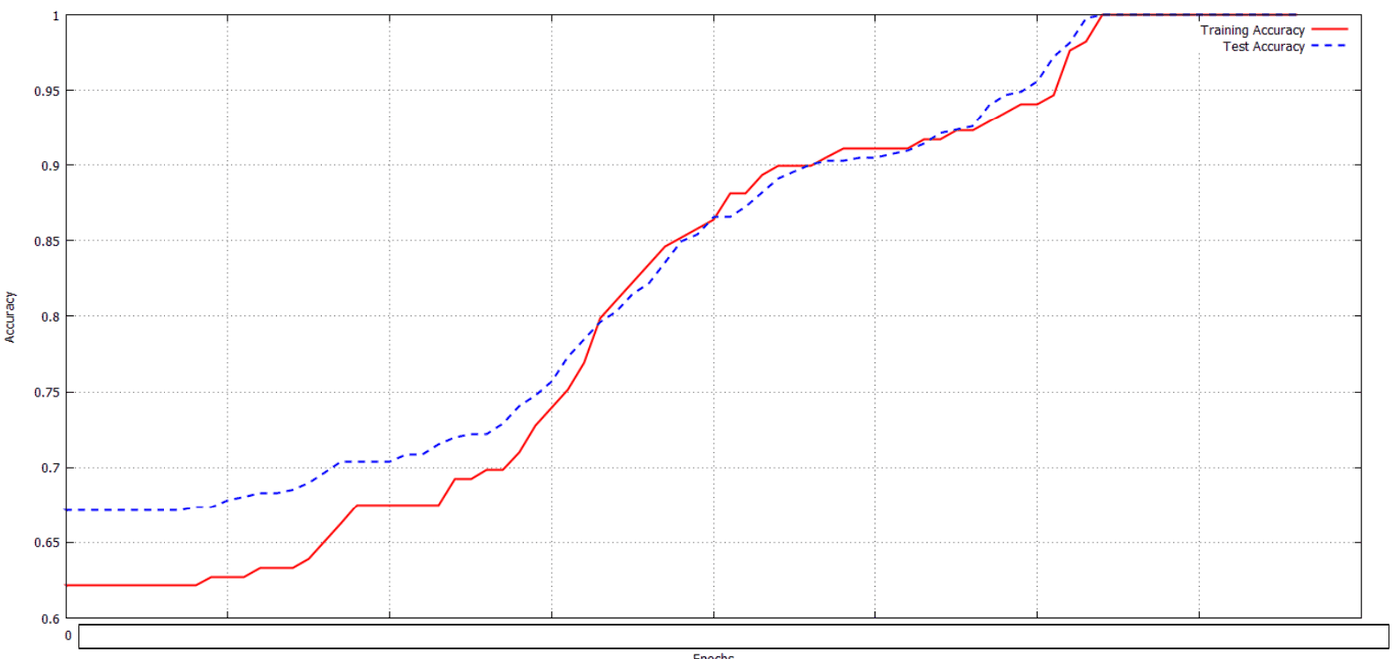
\includegraphics[width=0.80\linewidth,height=0.42\textheight,keepaspectratio]{images/08-nn2_monk2-acc.png}
\caption{MONK2: the accuracy reaches 100\% also on the test set (an
unusual case in general).}
\end{figure}

\begin{figure}[htbp]
\centering
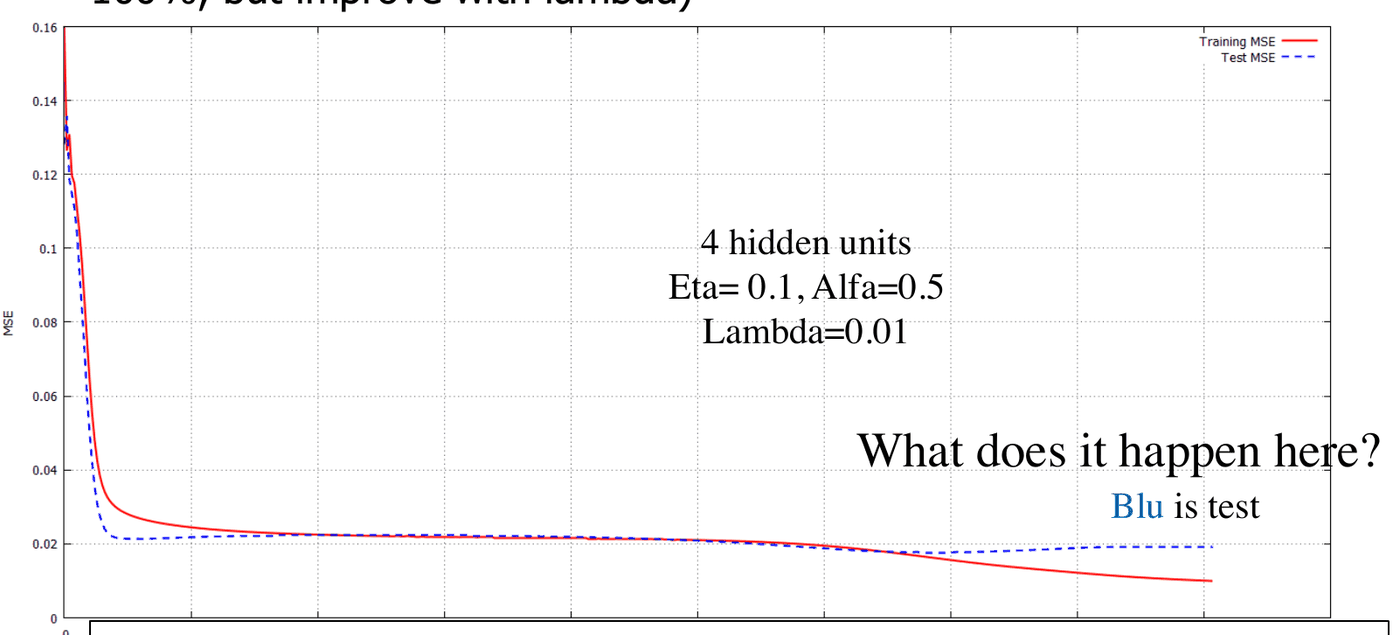
\includegraphics[width=0.80\linewidth,height=0.42\textheight,keepaspectratio]{images/08-nn2_monk3.png}
\caption{MONK3 with regularisation (\(\lambda = 0.01\)): MONK3 contains
noise and can overfit; the test does not reach 100\%.}
\end{figure}

\begin{boxquestion}{What happens in Fig.\ 8.13?}

In the final part the training error keeps decreasing while the test
error rises slightly: it is the onset of \textbf{overfitting} (MONK3
has noisy labels). Regularisation mitigates it; a \(\lambda\) chosen
with model selection or early stopping would help.

\end{boxquestion}

To verify backpropagation one can use a step-by-step example (beware if
it omits the biases) or a reliable library as an ``oracle'' (Keras,
scikit-learn, PyTorch\ldots). Other useful datasets can be found in the
UCI Machine Learning Repository.

\begin{boxnote}{Project preview (A.Y. 2026/27 rules)}

In past years the project was mandatory (groups of 2--3, type A with a
simulator implemented from scratch or type B with libraries, ML-CUP
competition). From A.Y. 2026/27 the project is \textbf{optional}:
groups of \textbf{2 students}, implementation/application/analysis of
an ML method with experimental evaluation, presented as a
\textbf{poster} in one of the last lectures (December). It can give a
small bonus but it is not necessary for the exam, which is based on the
written test (see
\href{01\%20-\%20Introduzione\%20al\%20Machine\%20Learning}{01 -
Introduction to Machine Learning}). The advice on MONK remains valid as
a test of any implementation.

\end{boxnote}

\begin{boxquestion}{Possible exam questions}

\begin{itemize}
\tightlist
\item
  How are the weights initialised and why?
\item
  Differences between on-line, batch and mini-batch.
\item
  Role of the learning rate; what is momentum and why does it work?
\item
  Is it necessary to find the global minimum? Why?
\item
  How does overfitting manifest itself in a neural network? What is
  early stopping?
\item
  Write the loss with weight decay and the update rule with momentum.
\item
  Does regularisation improve the stability of convergence?
\item
  Describe Cascade Correlation.
\item
  How are inputs and outputs represented for regression and
  classification?
\end{itemize}

\end{boxquestion}
